\chapter{Trabajo relacionado} \label{chapter:chapter2}

\section{WiNER: Un corpus anotado de Wikipedia para Reconocimiento de Entidades Nombradas}

Como se mencionó previamente, en esta tesis se estudiará el impacto de una técnica de aprendizaje semi-supervisado, redes convolucionales en escalera, en una tarea de reconocimiento de entidades nombradas. Para eso se buscó un recurso de referencia que pudiera servirnos a la hora de establecer una base de experimentos en donde evaluar las redes en escalera.

Si bien hay varias opciones disponibles para estudiar, muchas de ellas eran pagas o bien requerían un proceso de registro que llevaba mucho tiempo. Es por eso que se decidió trabajar con la Wikipedia como base. Ahora bien, una opción sería hacer todo el trabajo de preproceso y diseñar el corpus de base para los experimentos. Sin embargo, eso también consume mucho tiempo.
 
Convertir Wikipedia en un corpus de entidades nombradas anotadas con tipos es una tarea que recibió cierta atención a lo largo de los últimos años. En particular, en el trabajo de \cite{WiNER-Ghaddar-Langlais} se propuso una nueva metodología aplicada a la Wikipedia en inglés para construir WiNER, un gran corpus anotado de alta calidad. 

Para realizar esto aplicaron un pipeline de anotación, el cual consta de tres etapas. En primera instancia se consideran los enlaces directos de cada artículo objetivo, buscando en su texto los títulos de los artículos que se acceden. A su vez, cuentan con un recurso previo\footnote{\url{http://rali.iro.umontreal.ca/rali/en/}} que enumera todas las menciones del texto que se refieren al concepto principal de un artículo. Esto posibilita realizar una relación entre las correferencias del recurso y los títulos accedidos. A cada una de estas coincidencias se le asigna una etiqueta con la entidad asociada proveniente de una tabla de correferencias. 

Con el fin de obtener una mayor cobertura, en una segunda etapa ya se consideran enlaces anidados, buscando en el artículo objetivo los títulos de los artículos alcanzados y en caso de haber coincidencias se les asignan las entidades nombradas correspondientes. Finalmente, estos títulos emparejados en la segunda etapa también se comparan con sus menciones en la tabla de correferencias.

En cuanto a la evaluación del corpus generado, por un lado se realiza una evaluación manual a partir de un subconjunto de 1000 menciones. En esta etapa se mide la exactitud (o \textit{accuracy} en inglés) obtenida luego de aplicar cada etapa del pipeline. 

Posteriormente, se utilizan otros corpus de entidades anotadas, entre ellos uno clásico de referencia, el CONLL-2003 obtenido en el trabajo de \cite{TjongKimSang:2003:ICS:1119176.1119195}. Se compara el desempeño de distintos modelos con la métrica F1-score sobre las clases para nombres de personas (PER), organizaciones (ORG) y lugares (LOC) donde lo que varía fijado un modelo es la proporción del corpus WiNER que se utiliza y el corpus de evaluación, siendo el modelo LSTM-CRF \cite{DBLP:journals/corr/HuangXY15} el más prometedor.

\section{Embeddings para desambiguación del sentido de palabras}

Uno de los problemas fundamentales a la hora de lidiar con algoritmos de aprendizaje automático es la manera de representar los datos. Esto se debe a que los algoritmos esperan como entrada un vector de números de tamaño fijo. E.g., las imágenes pueden representarse mediante la intensidad de cada uno de sus píxeles. 

En el caso del trabajo con texto, la representación de los datos es algo particularmente complejo. Principalmente se debe a la naturaleza discreta de las palabras, donde las representaciones clásicas suelen ser ralas (i.e. vectores de mucha dimensionalidad, pero con muchos ceros). 

Ejemplos de este tipo de representaciones son los vectores \textit{one-hot encodings}. Para estos casos cada vector tiene la dimensionalidad del total de palabras del vocabulario, donde cada palabra se corresponde con una componente del vector. Entonces cada palabra es representada por un vector de todos 0's salvo un 1 en la componente que tenga asociada. Dado que el tamaño del vocabulario en general es considerablemente grande provoca que estos vectores sean de gran dimensionalidad. Además, hay que notar que los vectores no preservan información sobre el contexto en el que sucedieron las palabras en el texto, sino que son representaciones discretas de las mismas.

Hace unos años comenzaron a utilizarse más las representaciones distribuidas de las palabras, donde cada palabra es representada por las palabras de su vecindad. En particular, aparecieron los \textit{word embeddings}, vectores densos y continuos que codifican la probabilidad de una palabra dada su vecindad. 

Existen diferentes métodos para obtener \text{word embeddings}, pero todos tienen el objetivo de generar representaciones de palabras a partir de un corpus sin etiquetas.

En particular, el algoritmo Word2Vec \cite{DBLP:journals/corr/MikolovSCCD13}, explora dos arquitecturas de modelos basados en una red neuronal que buscan codificar la probabilidad de ocurrencia de una palabra dado su contexto. Esta red es entrenada con un gran corpus y las proyecciones son los word embeddings que el modelo Word2Vec produce. Aún así, los embeddings de palabras sólo representan palabras. Todavía queda el problema de cómo representar oraciones de palabras.

En el trabajo de \cite{iacobacci-etal-2016-embeddings} se estudia cómo los embeddings de palabras pueden ser utilizados para la tarea de Desambiguación del Sentido de las Palabras (del inglés \textit{Word Sense Disambiguation}). En particular, este estudio considera cuatro estrategias diferentes para integrar un modelo de word embeddings pre-entrenado en un sistema supervisado de desambiguación de sentidos: concatenación, promedio, decaimiento fraccional y decaimiento exponencial. Con estas estrategias se busca obtener una representación más informativa de cada palabra de acuerdo al contexto en la que ocurre. 

El framework que utilizaron para la desambiguación de sentidos es \textit{It Makes Sence (IMS)} \cite{Zhong:2010:MSW:1858933.1858947}, el cual provee una plataforma extensible y flexible para la desambiguación de sentidos supervisada que permite la verificación de diferentes características (entre ellas \textit{POS tagging}\footnote{\url{https://en.wikipedia.org/wiki/Part-of-speech_tagging}}) y técnicas de clasificación. IMS utiliza como clasificador un modelo de \textit{Support Vector Machine}\footnote{\url{https://en.wikipedia.org/wiki/Support-vector_machine}} con kernel lineal.

Se realiza una evaluación de los embeddings propuestos en base a dos tareas estándar de desambiguación de sentidos: \textit{lexical sample} y \textit{all-words}. El objetivo de la primera tarea es que el sistema IMS analice los contextos de los sentidos individuales de un pequeño conjunto de palabras anotadas y capture pistas que puedan usarse para distinguir diferentes sentidos de una palabra en la fase de test. El objetivo de la segunda tarea es desambiguar todas las palabras en un texto dado.

Estudiar este trabajo fue de gran interés sobretodo al comienzo de esta tesis ya que originalmente se había decidido encarar el problema de reconocimiento de entidades fijando que la entrada del modelo sea una palabra. Frente a esto, enriquecer la representación de cada palabra provista por el modelo Word2Vec con las palabras vecinas a fin de que cada instancia de entrenamiento cuente con información contextual tuvo mucho sentido. En particular, la estrategia de decaimiento exponencial resulta ser la más idónea correspondiendose con la intuición de que el impacto que tienen las palabras más cercanas a la palabra objetivo siempre es mayor y va disminuyendo a medida que se encuentran más distantes.


\section{Aprendizaje semi-supervisado con Redes en Escalera}
\label{sec:related_work_ladder}

Utilizar aprendizaje no supervisado con el fin de complementar al supervisado no es algo nuevo. Combinar una tarea auxiliar que ayude a entrenar una red neuronal fue propuesto por \cite{DBLP:conf/eurasip/SuddarthK90}. Al compartir las representaciones ocultas entre más de una tarea, la red generaliza mejor. Las redes neuronales en escalera son una combinación entre una red \textit{feedforward} y un \textit{autoencoder}. 

Una red neuronal feedforward tiene la particularidad de que las conexiones entre los nodos no forman un ciclo. Ejemplos de este tipo de redes neuronales son el perceptrón multicapa (ver Sección \ref{sec:perceptron}) y las redes convolucionales (ver Secciones \ref{sec:cnn:wide} y \ref{sec:cnn:deep}).

Por otra parte, un autoencoder es una red neuronal no supervisada, que tiene como objetivo reducir la dimensionalidad de una entrada mediante la reconstrucción de la misma. Este tipo de red está compuesta por un codificador (\textit{encoder}) encargado de comprimir la entrada en una representación espacial latente y un decodificador (\textit{decoder}), cuya tarea luego es reconstruir la entrada a partir de esta representación intermedia. La idea es que, el proceso de reducción de dimensiones obtendrá una representación que encuentre las propiedades más relevantes de los datos de entrenamiento.

En el modelo de red en escalera \cite{DBLP:journals/corr/Valpola14}, la tarea auxiliar es reducir el ruido de las representaciones en cada nivel del modelo. La estructura es un autoencoder con conexiones directas entre cada capa del codificador (\textit{encoder}) hacia el decodificador (\textit{decoder}) y la tarea de aprendizaje es similar a la de la reducción de ruido del autoencoder pero aplicados a cada capa, no solo a las entradas. 

Las conexiones entre las capas del codificador y el decodificador alivian la presión de representar detalles en las capas más internas en el modelo porque, a través de las mismas, el decodificador puede recuperar cualquier detalle descartado por el codificador. Esto es posible porque el decodificador utiliza la información sobre los costos en cada capa del pasaje limpio. 

Anteriormente, la red en escalera solo había sido aplicada en aprendizaje no supervisado \cite{DBLP:journals/corr/Valpola14}, en el trabajo de \cite{DBLP:journals/corr/RasmusVHBR15} el enfoque es combinar esto con aprendizaje supervisado. Los aspectos claves que plantea este nuevo enfoque son los siguientes:

\begin{description}
\item[Compatibilidad con métodos supervisados] La parte no supervisada se centra en los detalles relevantes encontrados por el aprendizaje supervisado. Además, se puede agregar a redes neuronales feedforward existentes, como por ejemplo el perceptrón multicapa o las redes neuronales convolucionales.

\item[Escalabilidad resultante del aprendizaje local] Además de un objetivo de aprendizaje supervisado en la capa superior, el modelo tiene objetivos de aprendizaje no supervisado locales en cada capa, por lo que es adecuado para redes neuronales muy profundas.

\item[Eficiencia computacional] La parte del codificador del modelo corresponde al aprendizaje supervisado normal. Al agregar un decodificador, se triplica aproximadamente el cálculo durante el entrenamiento, pero no necesariamente el tiempo de entrenamiento, ya que el mismo resultado se puede lograr más rápido a través de una mejor utilización de la información disponible. En general, el cálculo por actualización escala de manera similar a cualquier enfoque de aprendizaje supervisado, con un pequeño factor multiplicativo.
\end{description}

En la red en escalera el proceso de inferencia puede ser aprendido usando el principio de reducción de ruido, que ha sido utilizado, por ejemplo, en autoencoders que reducen ruido (en siglas: {\em dAE}, del inglés \textit{denoising autoencoders}), y en separación de fuente con reducción de ruido (en siglas: {\em DSS}, del inglés \textit{denoising source separation}).

En dAE, un autoencoder es entrenado para reconstruir la observación original \textbf{x} a partir de una versión corrupta $\tilde{\textbf{x}}$. El aprendizaje se basa simplemente en minimizar la norma de la diferencia de la \textbf{x} original y su reconstrucción $\hat{\textbf{x}}$ de $\tilde{\textbf{x}}$; el costo a minimizar es, entonces $\|\hat{\textbf{x}} - \textbf{x}\|^2$.

\begin{figure}[h!]
\begin{center}
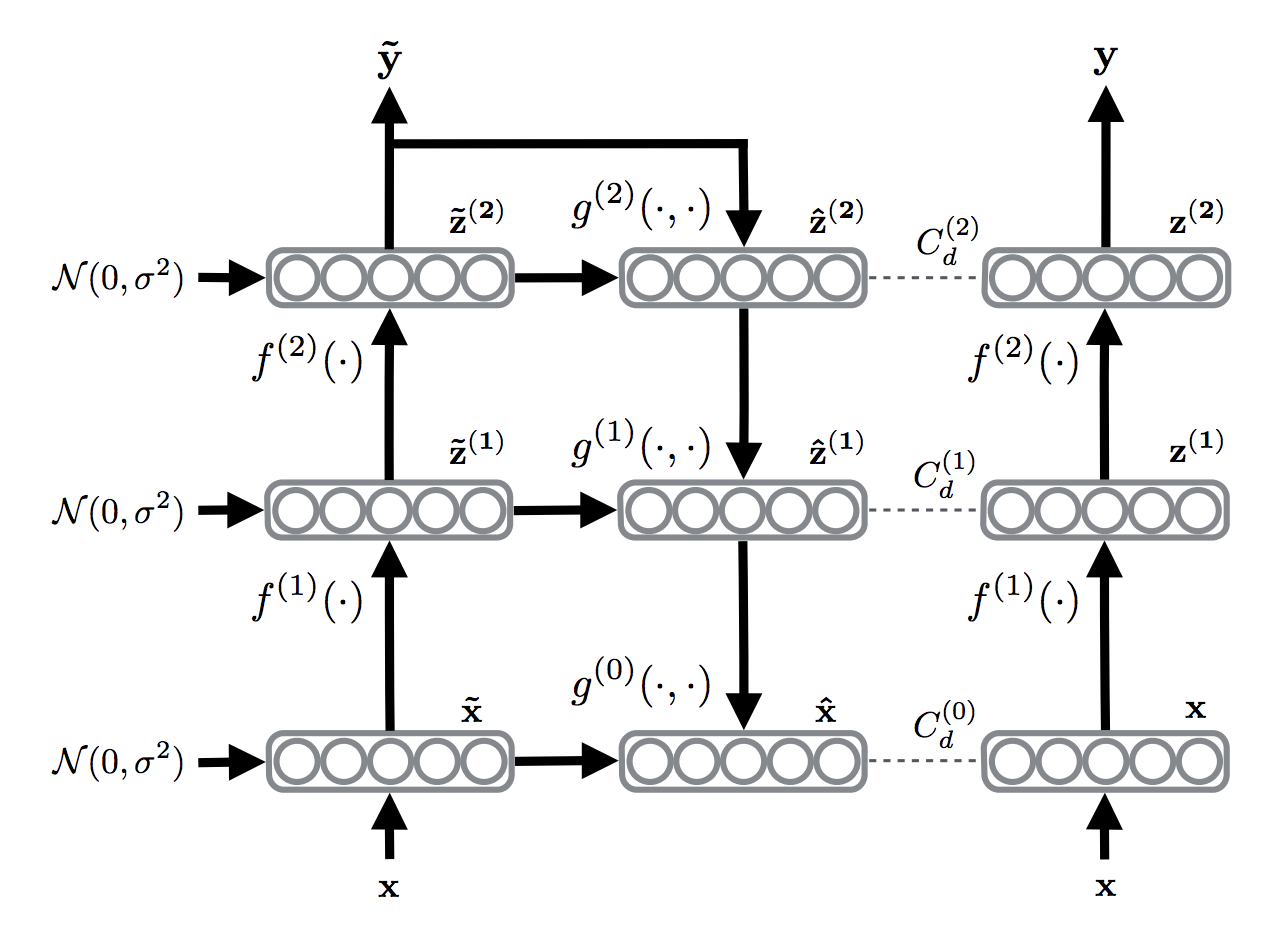
\includegraphics[width=\textwidth]{images/ladder_architecture.png}
\caption{Ilustración conceptual de una red en escalera con L = 2 obtenida del trabajo de \cite{DBLP:journals/corr/RasmusVHBR15}. El camino feedforward $(\textbf{x}\rightarrow\textbf{z}^{(1)}\rightarrow\textbf{z}^{(2)}\rightarrow\textbf{y})$ comparte las asignaciones $f^{(l)}$ con el camino feedforward corrupto, o codificador $(\textbf{x}\rightarrow\tilde{\textbf{z}}^{(1)}\rightarrow\tilde{\textbf{z}}^{(2)}\rightarrow\tilde{\textbf{y}})$. El decodificador $(\tilde{\textbf{z}}^{(l)}\rightarrow\hat{\textbf{z}}^{(l)}\rightarrow\hat{\textbf{x}})$ consiste en las funciones de reducción de ruido $g^{(l)}$ y tiene funciones de costo $C_{d}^{(l)}$ en cada capa, tratando de minimizar la diferencia entre $\hat{\textbf{z}}^{(l)}$ y $\textbf{z}^{(l)}$.
La salida $\tilde{\textbf{y}}$ del codificador también se puede entrenar para que coincida con las etiquetas disponibles $t(n)$. }
\label{fig:ladder_architecture}
\end{center}
\end{figure}


Mientras que las dAE normalmente sólo están capacitadas para reducir el ruido de las observaciones, las DSS se basan en la idea de utilizar funciones de reducción de ruido $\hat{\textbf{z}} = g(\textbf{z})$ de las variables latentes \textbf{z} para entrenar una función $f(\textbf{x}) = \textbf{z}$ que modela la probabilidad de las variables latentes en función de las observaciones. La función de costo es idéntica a la usada en un dAE salvo el hecho de que las variables latentes \textbf{z} reemplazan a las observaciones \textbf{x}; esto es, $\|\hat{\textbf{z}} - \textbf{z}\|^2$. Lo único que hay que tener en cuenta es que \textbf{z} debe normalizarse de alguna manera, ya que de lo contrario el modelo tiene una solución trivial $\textbf{z} = \hat{\textbf{z}} = constante$. En un dAE esto no puede suceder ya que el modelo no puede cambiar la entrada \textbf{x}.

La Figura \ref{fig:ladder_architecture} muestra la estructura de una red en escalera. Cada capa $(l)$ contribuye, a la función de costo $C_{d}$, un término de la forma $C_{d}^{(l)} = \| \textbf{z}^{(l)} - \hat{\textbf{z}}^{(l)}\|^2$ que entrena las capas superiores (tanto codificador como decodificador), para aprender la función de reducción de ruido $\hat{\textbf{z}}^{(l)} = g^{(l)}(\tilde{\textbf{z}}^{(l)},\hat{\textbf{z}}^{(l+1)})$ que asigna el valor corrupto $\tilde{\textbf{z}}^{(l)}$ al estimador de reducción de ruido $\hat{\textbf{z}}^{(l)}$. Como la estimación $\hat{\textbf{z}}^{(l)}$ incorpora todo el conocimiento previo sobre \textbf{z}, el mismo término de función de costo también entrena las capas del codificador, con el objetivo de encontrar características más limpias que coincidan mejor con el valor esperado previo.

Dado que la función de costo necesita tanto lo limpio $\textbf{z}^{(l)}$ como lo corrupto $\tilde{\textbf{z}}^{(l)}$, durante el entrenamiento el codificador se ejecuta dos veces: un pasaje limpio por $\textbf{z}^{(l)}$ y un pasaje corrupto por $\tilde{\textbf{z}}^{(l)}$.

Una forma de visualizar la red en escalera es considerarla como una colección de autoencoders anidados que comparten partes de la maquinaria de reducción de ruido entre sí. Desde el punto de vista del autoencoder en la capa \textit{l}, las representaciones de las capas superiores se pueden tratar como neuronas ocultas. En otras palabras, no hay una razón particular por la cual $\hat{\textbf{z}}^{(l+i)}$ producido por el decodificador, deba parecerse a la correspondiente representación $\textbf{z}^{(l+i)}$ producida por el codificador. Solo la función de costo $C_{d}^{(l+i)}$ los une y obliga a la inferencia a proceder en orden inverso en el decodificador. Este intercambio ayuda a un autoencoder de reducción de ruido profundo a aprender el proceso de reducción de ruido a medida que divide la tarea en subtareas significativas de reducción de ruido en representaciones intermedias.